\section{Experiments}
\label{sec:exp}

\begin{table*}[!t]
\centering
\caption{
Results on the LIBERO benchmark \cite{liu2023libero}.
We report per-suite success rates on the Spatial, Object, Goal, and Long suites, along with their average.
``Type'' distinguishes vision-language-action models (VLA) from world-action models (WAM).
Bold indicates the best result, and underline indicates the second best.
}
\label{tab:main_results}
\begingroup
\small
\setlength{\tabcolsep}{4pt}
\begin{tabular*}{0.78\textwidth}{@{\extracolsep{\fill}}lccccc|c}
\toprule
Method & Type & Spatial & Object & Goal & Long & Avg \\
\midrule
WorldVLA~\cite{worldvla} & WAM & 87.6 & 96.2 & 83.4 & 60.0 & 81.8 \\
GR00T-N1~\cite{bjorck2025gr00t} & VLA & 94.4 & 97.6 & 93.0 & 90.6 & 93.9 \\
$\pi_0$~\cite{BlackK-RSS-25} & VLA & 96.8 & 98.8 & 95.8 & 85.2 & 94.1 \\
GE-Act~\cite{genieenvisioner} & WAM & 98.2 & 97.6 & 95.8 & 94.4 & 96.5 \\
$\pi_{0.5}$~\cite{black2025pi} & VLA & \underline{98.6} & 98.2 & \underline{98.0} & 92.4 & 96.8 \\
OpenVLA-OFT~\cite{KimM1-RSS-25} & VLA & 97.6 & 98.4 & 97.9 & 94.5 & 97.1 \\
FastWAM~\cite{fastwam} & WAM & 98.2 & \textbf{100.0} & 97.0 & 95.2 & 97.6 \\
Motus~\cite{bi2025motus} & WAM & 96.8 & \underline{99.8} & 96.6 & 97.6 & 97.7 \\
LingBot-VA~\cite{lingbotva} & WAM & 98.5 & 99.6 & 97.2 & \textbf{98.5} & \underline{98.5} \\
\midrule
\ourmethod (Ours) & WAM & \textbf{99.4} & 99.4 & \textbf{98.2} & \underline{97.8} & \textbf{98.7}\\
\bottomrule
\end{tabular*}
\endgroup
\end{table*}

\begin{table*}[!t]
\centering
\caption{
Results on LIBERO-Plus~\cite{liberoplus}.
Each column perturbs one factor of the original LIBERO tasks, and Avg is the success rate over all perturbed tasks.
``Init'' and ``BG'' denote the robot initial state and the background texture, respectively.
Bold indicates the best result, and underline indicates the second best.
}
\label{tab:liberoplus}
\begingroup
\small
\setlength{\tabcolsep}{4pt}
\begin{tabular*}{0.78\textwidth}{@{\extracolsep{\fill}}lccccccc|c}
\toprule
Method & Layout & Camera & Init & Language & Light & BG & Noise & Avg \\
\midrule
OpenVLA~\cite{kim2024openvla} & 28.5 & 0.8 & 3.5 & 23.0 & 8.1 & 34.8 & 15.2 & 15.6 \\
WorldVLA~\cite{worldvla} & 38.0 & 0.1 & 27.9 & 41.6 & 43.7 & 17.1 & 10.9 & 25.0 \\
NORA~\cite{nora} & 62.1 & 2.2 & 37.0 & 65.1 & 45.7 & 58.6 & 12.8 & 39.0 \\
UniVLA~\cite{univla} & 31.9 & 1.8 & 46.2 & 69.6 & 69.0 & 81.0 & 21.2 & 43.9 \\
FastWAM~\cite{fastwam} & 60.7 & 16.4 & 44.5 & 68.9 & 78.2 & 53.7 & 37.7 & 50.0 \\
$\pi_0$~\cite{BlackK-RSS-25} & 68.9 & 13.8 & 6.0 & 58.8 & 85.0 & 81.4 & 79.0 & 53.6 \\
$\pi_0$-FAST~\cite{pi0fast} & 68.8 & \textbf{65.1} & 21.6 & 61.0 & 73.2 & 73.2 & 74.4 & 61.6 \\
OpenVLA-OFT~\cite{KimM1-RSS-25} & 74.2 & \underline{56.4} & 31.9 & \underline{79.5} & 88.7 & \textbf{93.3} & 75.8 & 69.6 \\
GE-Act~\cite{genieenvisioner} & \underline{83.0} & {49.6} & \underline{77.2} & 79.4 & \underline{94.8} & 85.1 & \underline{83.0} & \underline{77.8} \\
\midrule
\ourmethod (Ours) & \textbf{85.3} & 54.8 & \textbf{78.3} & \textbf{81.7} & \textbf{96.5} & \underline{88.9} & \textbf{90.7} & \textbf{81.3}\\
\bottomrule
\end{tabular*}
\endgroup
\end{table*}

We comprehensively evaluate \ourmethod across both simulation benchmarks and a real-world robot platform.
We organize the experiments around four questions:

\begin{itemize}
    \item \textbf{Q1:} Does \ourmethod achieve state-of-the-art performance on standard manipulation benchmarks and on a real robot?
    \item \textbf{Q2:} Does semantic foresight improve robustness when the environment or the instruction is perturbed?
    \item \textbf{Q3:} Does the predicted foresight actually steer future videos and actions generation to follow the instruction?
    \item \textbf{Q4:} How much does each component of \ourmethod contribute to the final performance?
\end{itemize}

\subsection{Experimental Setup}
\label{sec:exp_setup}

\paragraph{Benchmarks.}
We comprehensively evaluate \ourmethod on three benchmarks:
\begin{itemize}
    \item \textbf{LIBERO}~\cite{liu2023libero} evaluates tabletop manipulation on four suites (Spatial, Object, Goal, and Long).
    Following the standard protocol~\cite{kim2024openvla}, we evaluate 500 trials per suite and report the success rate.
    \item \textbf{LIBERO-Plus}~\cite{liberoplus} extends LIBERO with seven perturbation factors, covering object layout, camera viewpoint, robot initial state, language rephrasing, lighting, background texture, and sensor noise.
    \item \textbf{Real-world experiments} are conducted on an AgileX Cobot dual-arm platform, with the setup and tasks described in Sec.~\ref{sec:exp_realworld}.
\end{itemize}

\begin{figure*}[t]
    \centering
    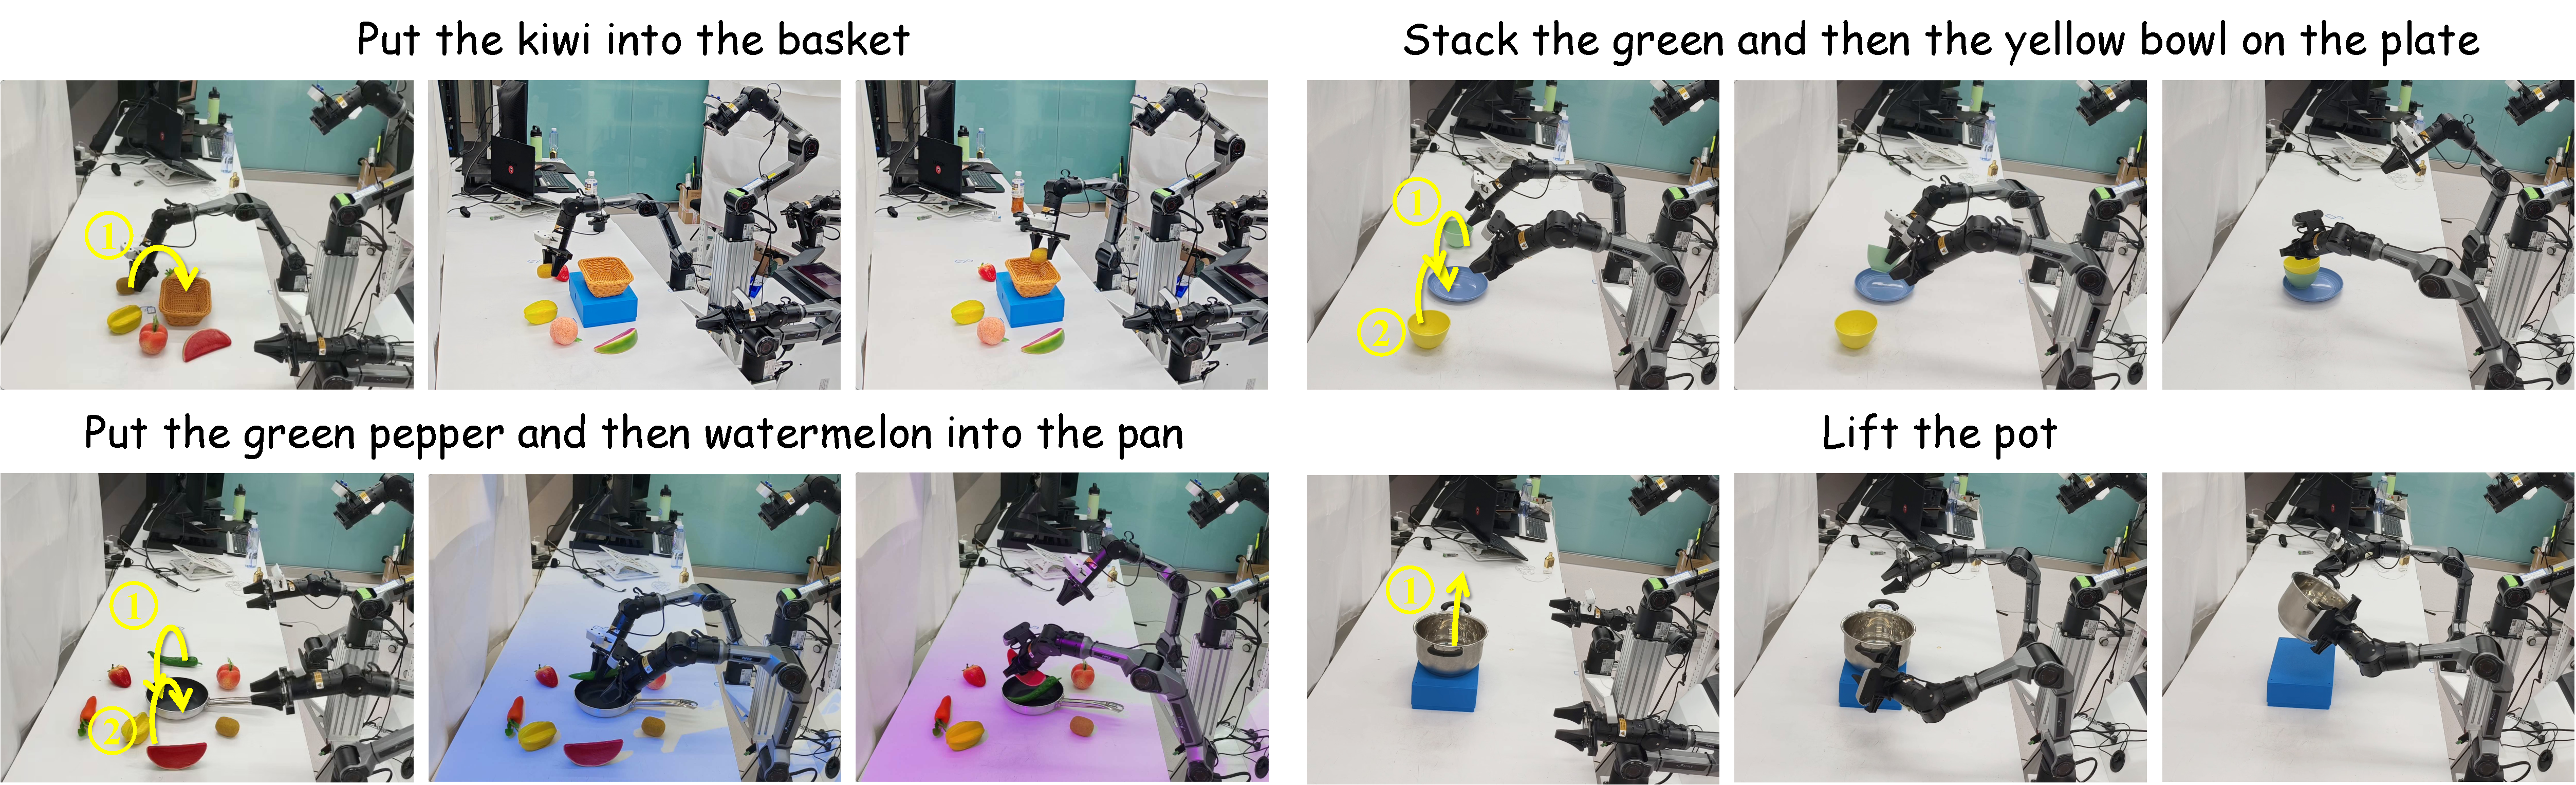
\includegraphics[width=\textwidth]{Figures/real_world.pdf}
    \caption{\textbf{Real-world qualitative results.} Qualitative execution sequences using our \ourmethod{} across four manipulation tasks, validating different generalization and manipulation capabilities: height generalization, stacking in the instructed order, target selection under distractors and lighting variation, and bimanual collaboration.}
    \label{fig:real_rollout}
\end{figure*}

\begin{figure}[t]
    \centering
    % Generated by scripts/plot_real_world.py; edit DATA and re-run to update.
    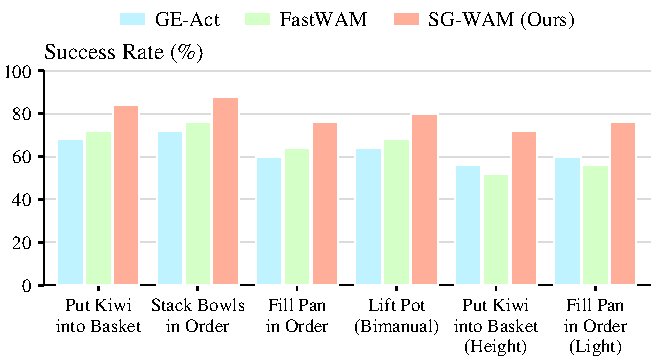
\includegraphics[width=\columnwidth]{Figures/real_results.pdf}
    \caption{\textbf{Real-world multi-task results.} We report success rates (SR) across four different tasks as well as two generalization experiments.  ``Height'' evaluates kiwi placement with the basket at a height unseen during data collection, while ``Light'' evaluates ordered pan filling under unseen lighting conditions.}
    \label{fig:realworld}
\end{figure}

\paragraph{Baselines.}
We compare against two groups of methods (see Table~\ref{tab:main_results}).
\textbf{VLA models}, including OpenVLA-OFT~\cite{KimM1-RSS-25}, $\pi_0$ and $\pi_{0.5}$~\cite{BlackK-RSS-25,black2025pi}, and GR00T-N1~\cite{bjorck2025gr00t}, map observations and instructions directly to actions without modeling future dynamics.
\textbf{WAM models}, including WorldVLA~\cite{worldvla}, GE-Act~\cite{genieenvisioner}, Motus~\cite{bi2025motus}, FastWAM~\cite{fastwam}, and LingBot-VA~\cite{lingbotva}, jointly predict future observations and actions but condition generation only on coarse text embeddings.


\paragraph{Implementation Details.}
Our \ourmethod utilizes Qwen3.5 2B~\cite{qwen35} as the semantic planner.
The two representation spaces we use are SigLIP2~\cite{siglip2} for text-grounded semantics and Depth Anything~3~\cite{lin2025depth} for spatial-aware semantics.
We align to the penultimate-layer patch tokens of SigLIP2 and to the last-layer features of Depth Anything~3. 
% Both feature maps use a $16{\times}16$ token grid, with feature dimensions of $1024$ and $2048$, respectively.
The planner predicts $K{=}4$ future keyframes at evenly spaced offsets, using $32$ shared base tokens together with $32$ query tokens per semantic branch.
\TODO{State the $K{=}4$ keyframe offsets (in future video frames and in control steps). Candidates found in code disagree; confirm which run the paper reports.}
% Evidence (2026-11-17 code audit, confirm before filling in):
%  (A) HPC3 SG-WAM qwen35_baton/config.py:43,56 + ge_act/configs/ltx_model/libero/action_model_libero_baton_stage3_hdf5.yaml:100:
%      offsets [0,3,5,8] of the T=9 future video frames (frame stride 36/9=4 steps) -> +4,+16,+24,+36 steps; NOT evenly spaced.
%  (B) W02 joint_vlm_geact_action_k4_50k/step_40000/joint_meta.json: offsets [2,4,6,8] (keyframe_offsets(9,4,'even_future')) -> +8,+16,+24,+32 steps; evenly spaced.
The world model is initialized from a pretrained LTX-Video~\cite{ltxvideo} diffusion model; the action expert is coupled to the video expert by joint attention as described in Sec.~\ref{sec:method_guidance}.
The model generates $T{=}9$ future frames and predicts an action chunk of $H{=}36$ steps via a flow-matching paradigm.
We conduct all three training stages on eight H100 GPUs.
Stage 1 runs for 20k steps with a learning rate of $4.2{\times}10^{-5}$ for the VLM and $4.2{\times}10^{-4}$ for the two resampler heads, weight decay $0.01$, and a cosine schedule with 2.5k warmup steps, where the spatial-aware term is weighted by $\lambda_{\mathrm{spa}}{=}4{\times}10^{-3}$.
Stages 2 and 3 each run for 30k steps with 1k warmup steps, using $2{\times}10^{-5}$ for the video expert, $1{\times}10^{-4}$ for the action expert, and $5{\times}10^{-5}$ for the semantic adapter, and retain the alignment term with $\lambda_{\mathrm{plan}}{=}0.25$ and the action term with $\lambda_{\mathrm{act}}{=}1.0$.
The semantic guidance is dropped with probability $0.15$ during training to enable classifier-free guidance at inference.
\TODO{Give the inference-time CFG scale and combination rule, or revise this claim: the audited LIBERO evaluation uses guidance scale $1.0$, i.e., no CFG at inference.}
% Evidence: HPC3 SG-WAM ge_act/experiments/eval_libero.py:353 (W02 copy :304) hard-codes guidance_scale=1.0; the pipeline enables CFG only for scale>1
% (custom_pipeline.py:655-656). The existing CFG path is TEXT CFG (empty negative prompt, eval_libero.py:345) combined as v_u + s*(v_c - v_u) on video and
% action at every step; the semantic plan is copied unchanged into both halves (custom_pipeline.py:178-181), so no semantic-guidance CFG is implemented.
% If no CFG is used, rewrite as: guidance dropout (p=0.15) is a training regularizer and inference uses the conditional prediction only.

\subsection{Comparisons with State-of-the-Art Methods (Q1 \& Q2)}
\label{sec:main_results}

\paragraph{Results on LIBERO.}
As shown in Table~\ref{tab:main_results}, \ourmethod achieves the highest average success rate of 98.7\% on LIBERO, surpassing the strongest baseline LingBot-VA (98.5\%).
For a direct comparison with the two baselines used in our real-world experiments, \ourmethod outperforms FastWAM and GE-Act by 1.1 and 2.2 points, respectively.

\paragraph{Robustness Under Perturbations.}
LIBERO-Plus perturbs one factor of the environment at a time (Table~\ref{tab:liberoplus}).
\ourmethod consistently outperforms competing baselines, reaching the highest average success rate of 81.3\% ($+3.5$ points), with a notable improvement under language perturbation (81.7\%, $+2.2$ points).
This gain highlights the advantage of grounding the instruction in the current observation.
While existing WAMs embed the instruction independently of the visual observation, \ourmethod predicts its semantic foresight from both the instruction and the current scene to yield guidance that stays grounded when the appearance or wording changes.

\begin{figure*}[!t]
    \centering
    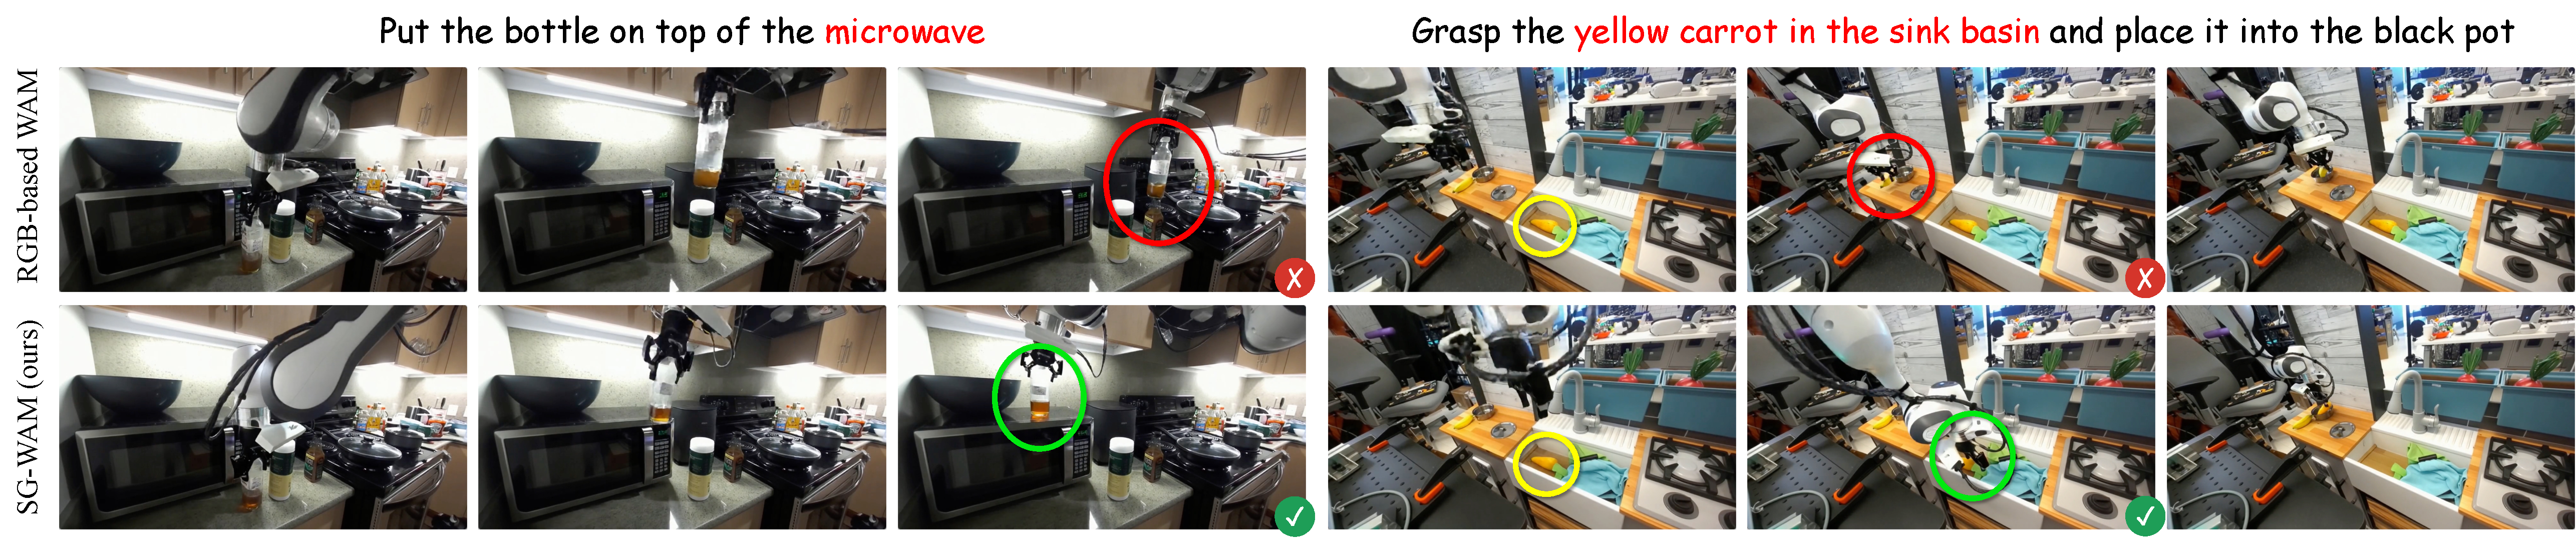
\includegraphics[width=\textwidth]{Figures/instruction.pdf}
    \caption{\textbf{Instruction-following comparison on DROID~\cite{droid}.} Videos generated from the same reference frame under out-of-distribution instructions, with the instructed target highlighted in red. For each instruction, the top row shows the RGB-based WAM and the bottom row shows \ourmethod, and red circles indicate the object or location acted upon.}
    \label{fig:if_vis}
\end{figure*}

\subsection{Multi-task Experiments in the Real World (Q1 \& Q2)}
\label{sec:exp_realworld}

\paragraph{Hardware Setup.}
We conduct real-world experiments on an AgileX Cobot dual-arm platform with two 6-DoF Piper arms, each equipped with a 1-DoF parallel gripper, so that both the robot state and the action are $14$-dimensional (six joints and one gripper per arm).
Three Orbbec Dabai DC1 cameras provide the visual input: one front-facing camera as Eye-on-Base and one camera on each wrist as Eye-on-Hand, all recording $640{\times}480$ RGB images at $30$\,fps; depth is not used.
Demonstrations are collected through master--puppet teleoperation at $30$\,Hz, which also defines the time step of the recorded observations and actions, while the low-level arm controller runs at $200$\,Hz.
At test time, the policy follows the receding-horizon execution described in Sec.~\ref{sec:method_deploy}.
GE-Act and FastWAM are fine-tuned on the same demonstrations and receive the same camera views; each keeps the action-chunk configuration of its official release, with FastWAM following its dual-arm RoboTwin setting, so the comparison differs only in the conditioning of generation.

\paragraph{Tasks.}
We select four representative tasks (see Figure~\ref{fig:real_rollout}): Put kiwi into basket, Stack bowls in order, Fill pan in order, and Lift pot.
Each task involves multiple distractor objects and randomized initial layouts, and the pick-and-place tasks specify both the target objects and the order in which they are placed.
We collect 100 teleoperated demonstrations per task, and each model is tested on each task with 50 trials, with object positions re-randomized between trials and the success rate as the performance metric.
For generalization, we further repeat the basket task at a container height unseen in the demonstrations and the pan task under lighting conditions that differ from data collection, again with 50 trials each and without any fine-tuning.

\begin{figure}[!t]
    \centering
    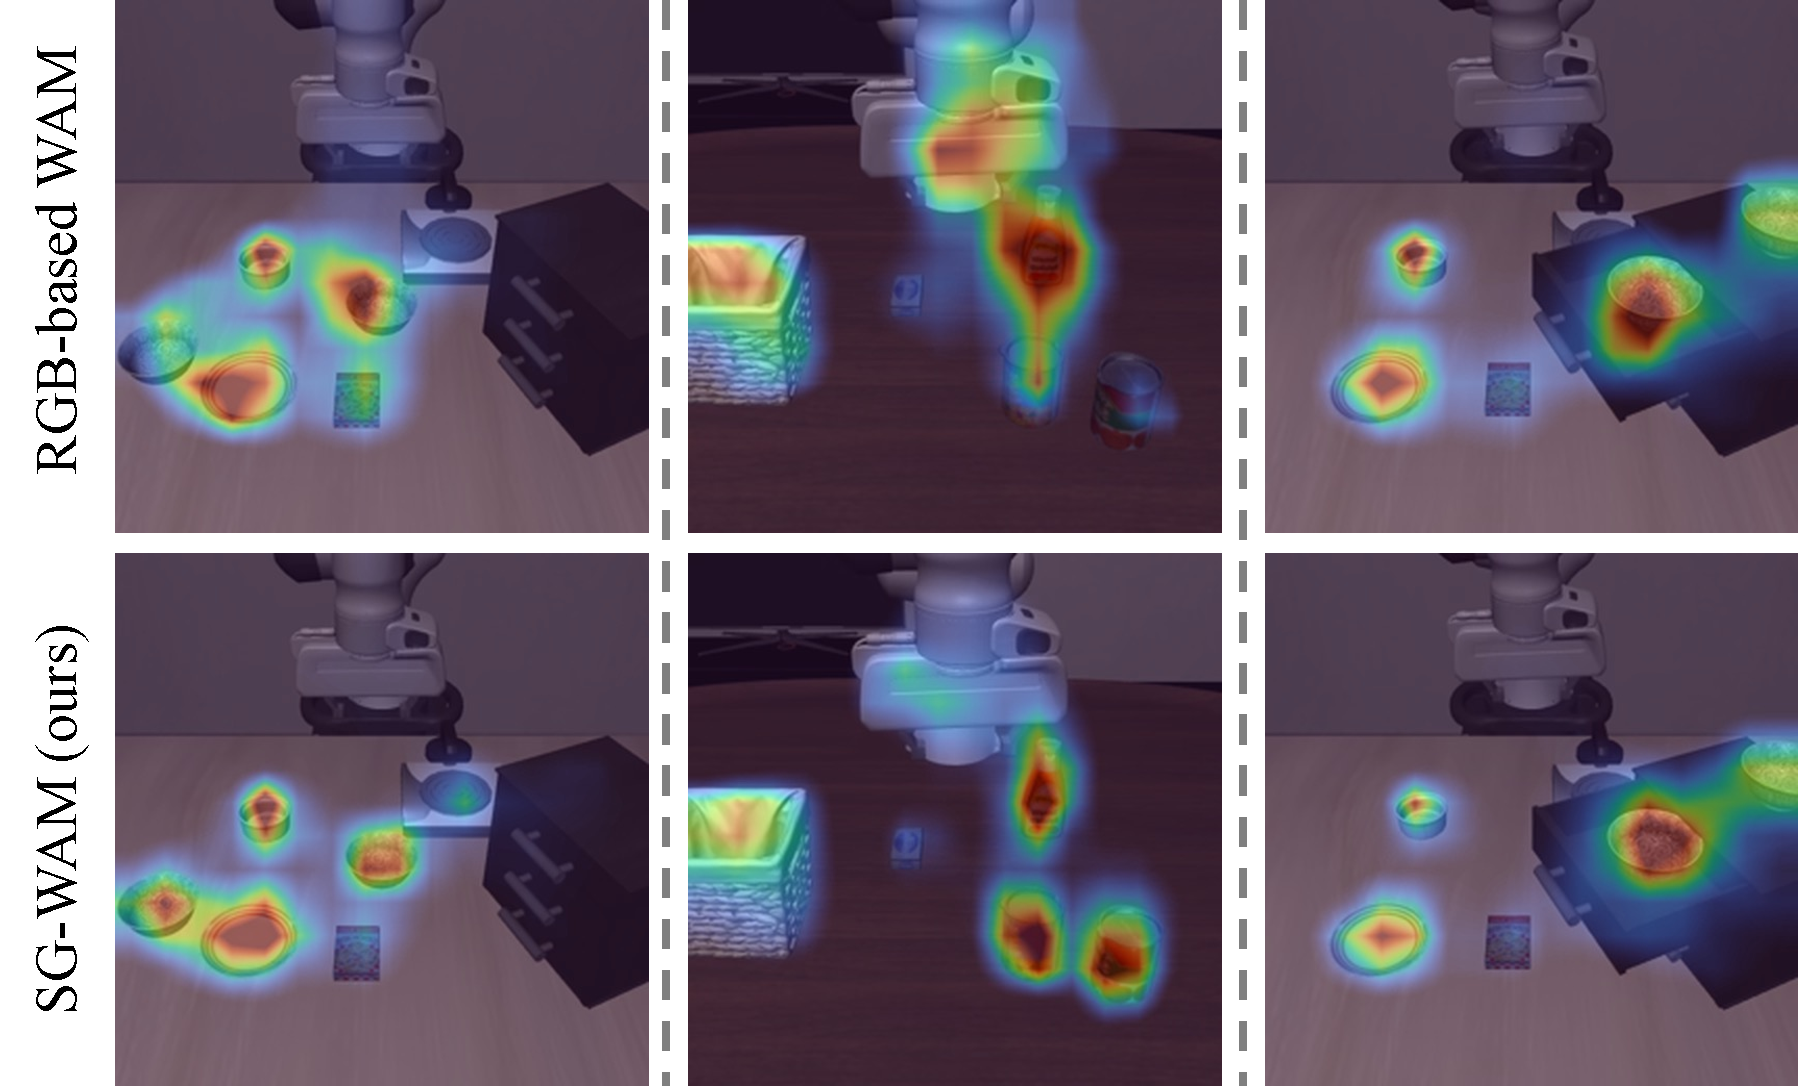
\includegraphics[width=\columnwidth]{Figures/Foresight.pdf}
    \caption{\textbf{Qualitative comparison of attention maps on LIBERO~\cite{liu2023libero}.} Action-to-video attention to the instruction-relevant object. The RGB-based WAM (top) spreads its attention over several objects and over the robot arm itself, while \ourmethod (bottom) concentrates it on the manipulated objects.}
    \label{fig:foresight_vis}
\end{figure}

\paragraph{Results.}
As shown in Figure~\ref{fig:realworld}, \ourmethod consistently outperforms GE-Act and FastWAM across the four standard tasks, achieving the highest success rate in each case.
The gain is largest on the tasks in which the instructed objects have to be selected among distractors and placed in the commanded order.
Notably, all policies are trained only on demonstrations collected in the standard setting, yet \ourmethod remains effective when the container is raised to a height never seen during data collection.
\ourmethod also attains the best success rate in both generalization settings, and its accuracy under the shifted lighting matches that of the standard pan task.
This result suggests that foresight represented in semantic feature space remains reliable under shifts in scene geometry or appearance.

\subsection{Instruction-Following Analysis (Q3)}
\label{sec:exp_instruction}

We next examine whether the foresight is what makes the generated futures and actions follow the instruction, using two qualitative studies.

\paragraph{Out-of-Distribution Instruction Following.}
We train both the RGB-based WAM and \ourmethod on DROID~\cite{droid}, and let them generate future videos from the same reference frame under instructions unseen during training.
As shown in Figure~\ref{fig:if_vis}, the RGB-based WAM places the bottle on the stove instead of the microwave, and reaches for the wrong item instead of the carrot in the sink basin, while \ourmethod acts on the commanded object in both cases.
The RGB-based WAM receives an instruction embedding computed independently of the observation, and therefore relies mainly on visual cues, drifting toward the most salient object when the wording is unfamiliar.

\paragraph{Instruction-Grounded Attention Analysis.}
\TODO{Specify the model, layers, heads, query/key tokens and aggregation used for Fig.~\ref{fig:foresight_vis}; the audited script does not match the current description.}
% Evidence: panels come from W02 VLA_WM/VLM4WAM/semantic_localization/wam_attention/generate_many.py (+ export_panels.py / make_wam_poster.py):
%  Cosmos-Predict2.5 FastWAM (SG: fastwam_sg_ckpt/.../step_015000.pt; RGB baseline: base DiT + SG text_proj), VIDEO-token -> TEXT-token cross-attention,
%  blocks 8/12/16/20, softmax over text keys, masked mean over valid text tokens, mean over heads, mean over the 4 layers, latent frame 0, 14x14 grid,
%  timestep 500, input = initial frame repeated 5x; post-process min-max, clip to 60-99th percentile, gamma 1.6, bilinear upsample, turbo colormap.
%  So it is neither the LTX model nor action->video attention. A true action->video script exists (W02 ltx_semantic_ckpt/sg_action_video.py:
%  all action_blocks[*].attn2, mean over heads and action queries, then layers, main view latent frame 4) but uses GT SigLIP2 plans.
As shown in Figure~\ref{fig:foresight_vis}, we compare the action-to-video attention heatmaps of \ourmethod against the RGB-based WAM.
The RGB-based WAM spreads its attention over several objects and over the robot arm itself, whereas \ourmethod concentrates it on the object named in the instruction, indicating that the guidance directs the capacity of the model to the task-relevant region.

\subsection{Ablation Study (Q4)}
\label{sec:exp_ablation}

To evaluate the individual contributions of the semantic guidance, the dual-semantic design, and the three-stage training, we train ablated variants on the same data setting with identical hyperparameters and evaluate them on LIBERO.
The results are summarized in Table~\ref{tab:ablation}.

\begin{table}[!t]
\centering
\caption{
Ablation study on the core design choices of \ourmethod.
We report the average success rate (\%) on LIBERO, where each row removes or replaces one component.
Bold indicates the best result.
}
\label{tab:ablation}
\begingroup
\small
\setlength{\tabcolsep}{4pt}
\begin{tabular}{lc}
\toprule
Variant & Success Rate (\%) \\
\midrule
\ourmethod (full) & \textbf{98.7} \\
\midrule
\multicolumn{2}{l}{\textit{Semantic guidance}} \\
\quad w/o semantic guidance & 97.2 \\
\multicolumn{2}{l}{\textit{Dual-semantics design}} \\
\quad w/o spatial-aware semantics & 98.3 \\
\quad w/o text-grounded semantics & 97.7 \\
\quad w/o shared semantic query tokens & 98.4 \\
\multicolumn{2}{l}{\textit{Three-stage training}} \\
\quad single-stage training & 97.9 \\
\bottomrule
\end{tabular}
\endgroup
\end{table}


\paragraph{Semantic Guidance.}
Removing the semantic guidance and conditioning the backbone on text alone causes the largest drop. This supports the benefit of instruction-grounded guidance for joint video-action generation.

\paragraph{Dual-Semantics Design.}
Removing either semantics degrades performance. The removal of text-grounded semantics causes a noticeable drop, since it decides which object to act on. The removal of spatial-aware semantics also leads to a drop, as it provides the geometry for manipulating that object.
This evidence supports the benefit of text-grounded and spatial-aware semantic guidance.
Replacing the shared query tokens with specific query tokens causes a small but consistent drop.

\paragraph{Three-Stage Training.}
Training the planner, the world model, and the action expert jointly from scratch also degrades performance.
The action expert then starts learning before the planner produces reliable guidance, which supports training the three components in stages.
